\documentclass[10pt,a4paper]{article}
\usepackage[english]{babel}
\usepackage{graphicx} 
\usepackage{amsmath}
\usepackage{amsfonts}
\usepackage{amssymb}
\usepackage{graphicx}
\usepackage{amstext}
\usepackage{scrlayer-scrpage}
\usepackage{titling}
\pagestyle{scrheadings}
\clearpairofpagestyles

\author{Emil Paulitz, Raphael Olipitz}
\title{Sequence Bioinformatics\\Assignment 05}
\begin{document}
	\ohead{\theauthor}
	\cfoot{\pagemark}
	\maketitle
	\section*{Task 2}
		\texttt{Partitions} is a tab to get an overview of the chosen alignments, ad choose or link their tree, clock model or site model. In \texttt{Tip Dates}, one can enter the sampling dates of the species, or let those get parsed automatically. In \texttt{Site Model}, one can specify the evolutionary model describing how the sequences arose, for example the Jukes-Cantor model (JC69) described in the lecture. The \texttt{clock model} panel allows to define the clock model used. This means, one can choose between different model of a molecular clock, assuming constant evolutionary rates at every point in time (strict clock) or varying time in different branches, depending on the model chosen. In \texttt{Priors}, the user is offered settings regarding the model of population growth, with parameters like birth rate. The \texttt{MCMC} tab shows the settings for the Markoff Chain Monte Carlo calculations like the chain length or length of the burn-in.
	\section*{Task 4}
		\begin{center}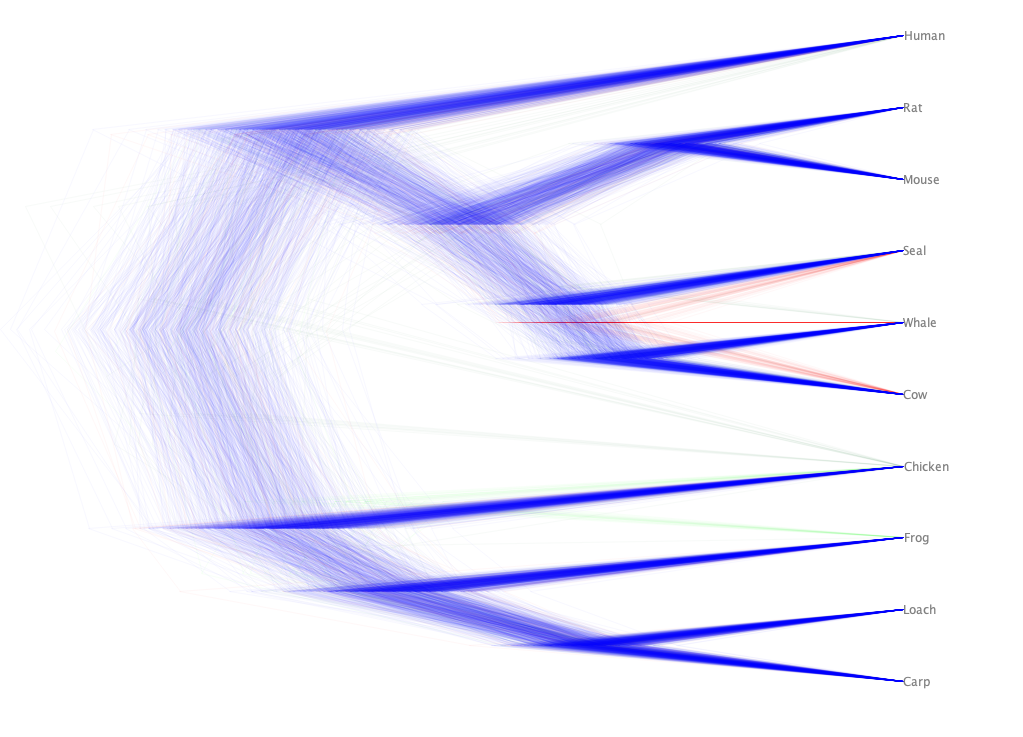
\includegraphics[width = 0.6\textwidth]{densi.png}\end{center}
		The visualization shows many superimposed trees. They seem to mostly agree on the general structure of the tree, placing for example rat and mouse relatively close, and grouping non-mammals, but do have different edge lengths. Because only the status in the present is known for sure, the farther the tree goes back in the past, the less certain predictions become. For example, the different trees diverge the most when predicting the point in time where mammals and non-mammals split up, which is the furthest in the past in this selection of species.
	\section*{Task 5}
		\begin{center}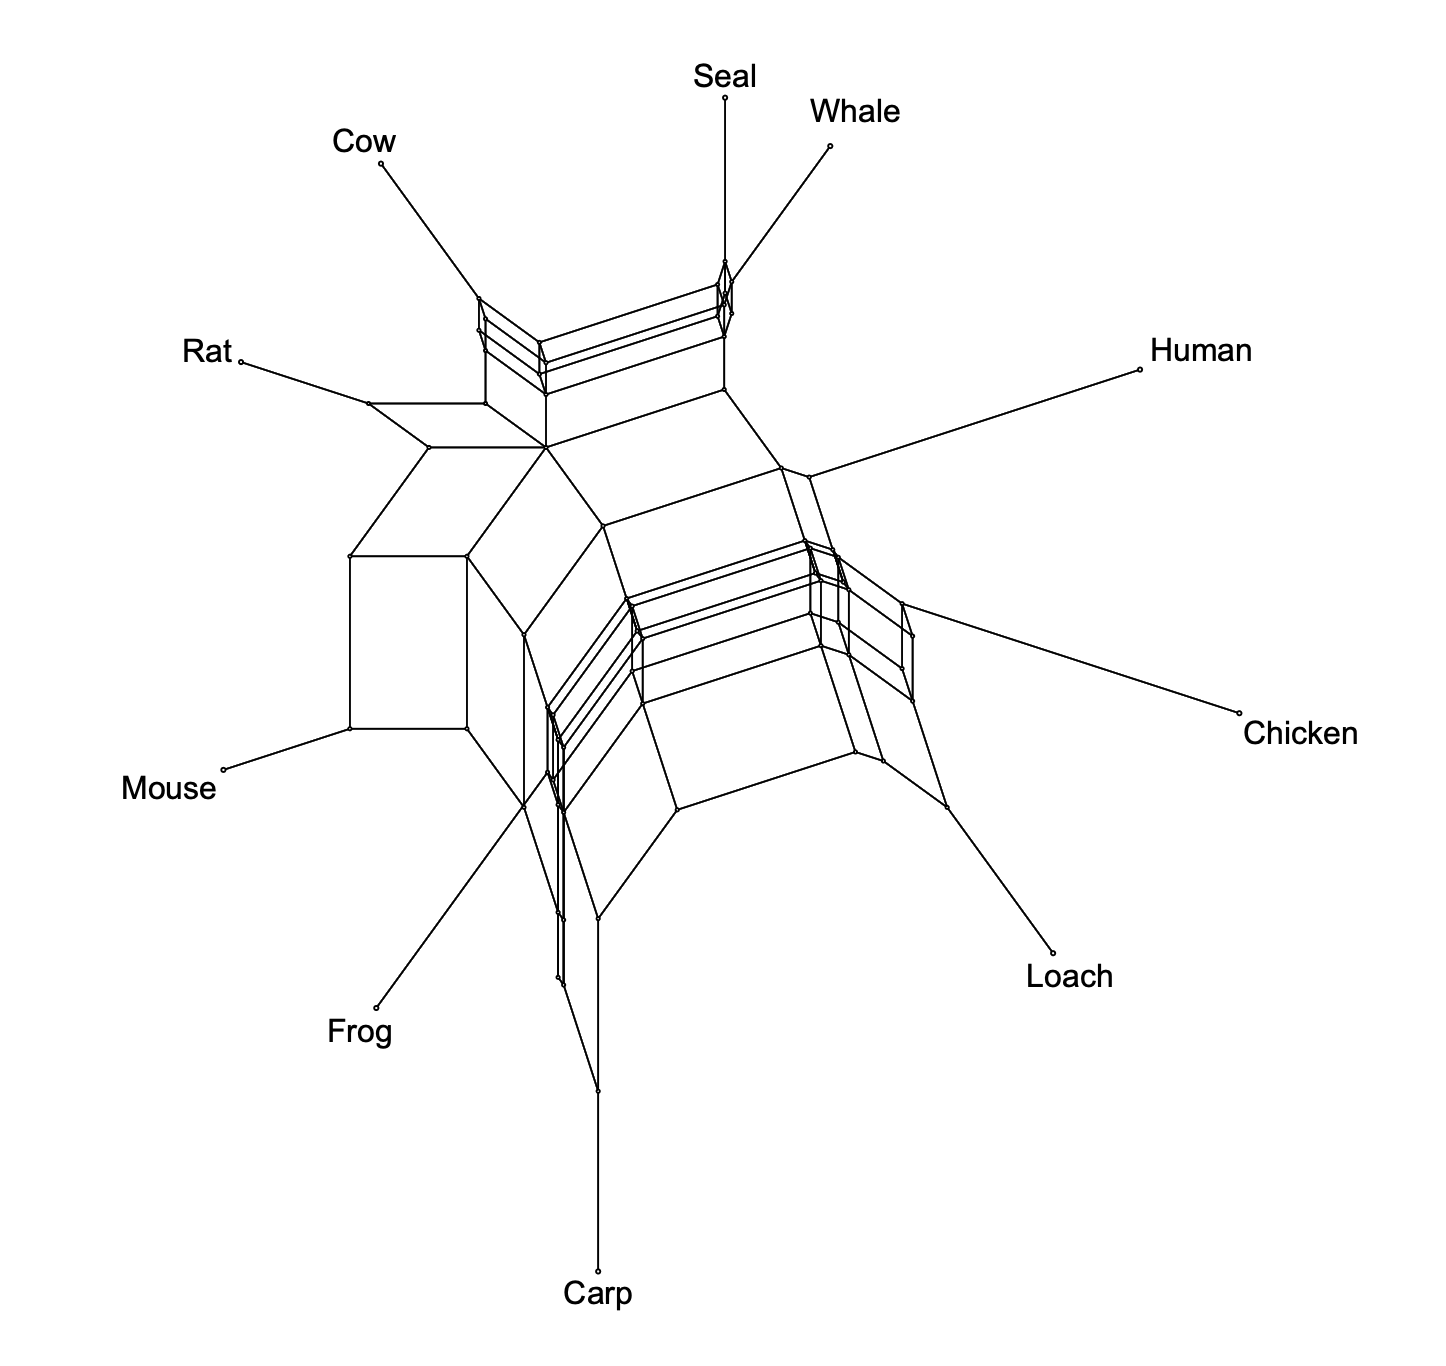
\includegraphics[width = 0.6\textwidth]{tree5.png}\end{center}
		The network depicts the different edge lengths of the generated trees all at once. One can for example see immediately how far one species is most certainly from all other species by the edge length that connects itself with the big web in the center. Humans and Chicken for example are far out. This is also confirmed by the DensiTree visualization. Seal and Whale on the other hand have a very short edge connecting them with the big web, and both are connected to the web in practically the same location, with multiple paths connecting them with a short distance. This suggests great evidence that these two species are closely related. 
	\section*{Task 6}
		\begin{figure}[h]
			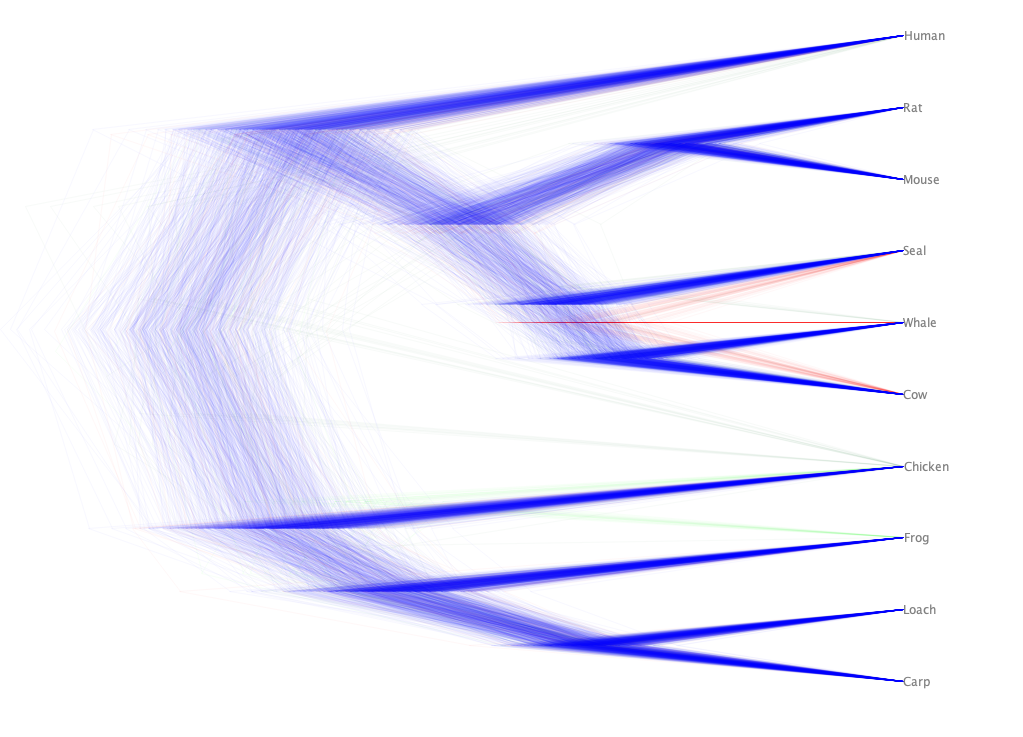
\includegraphics[width = 0.5\textwidth]{densi.png}%
			\hfill
			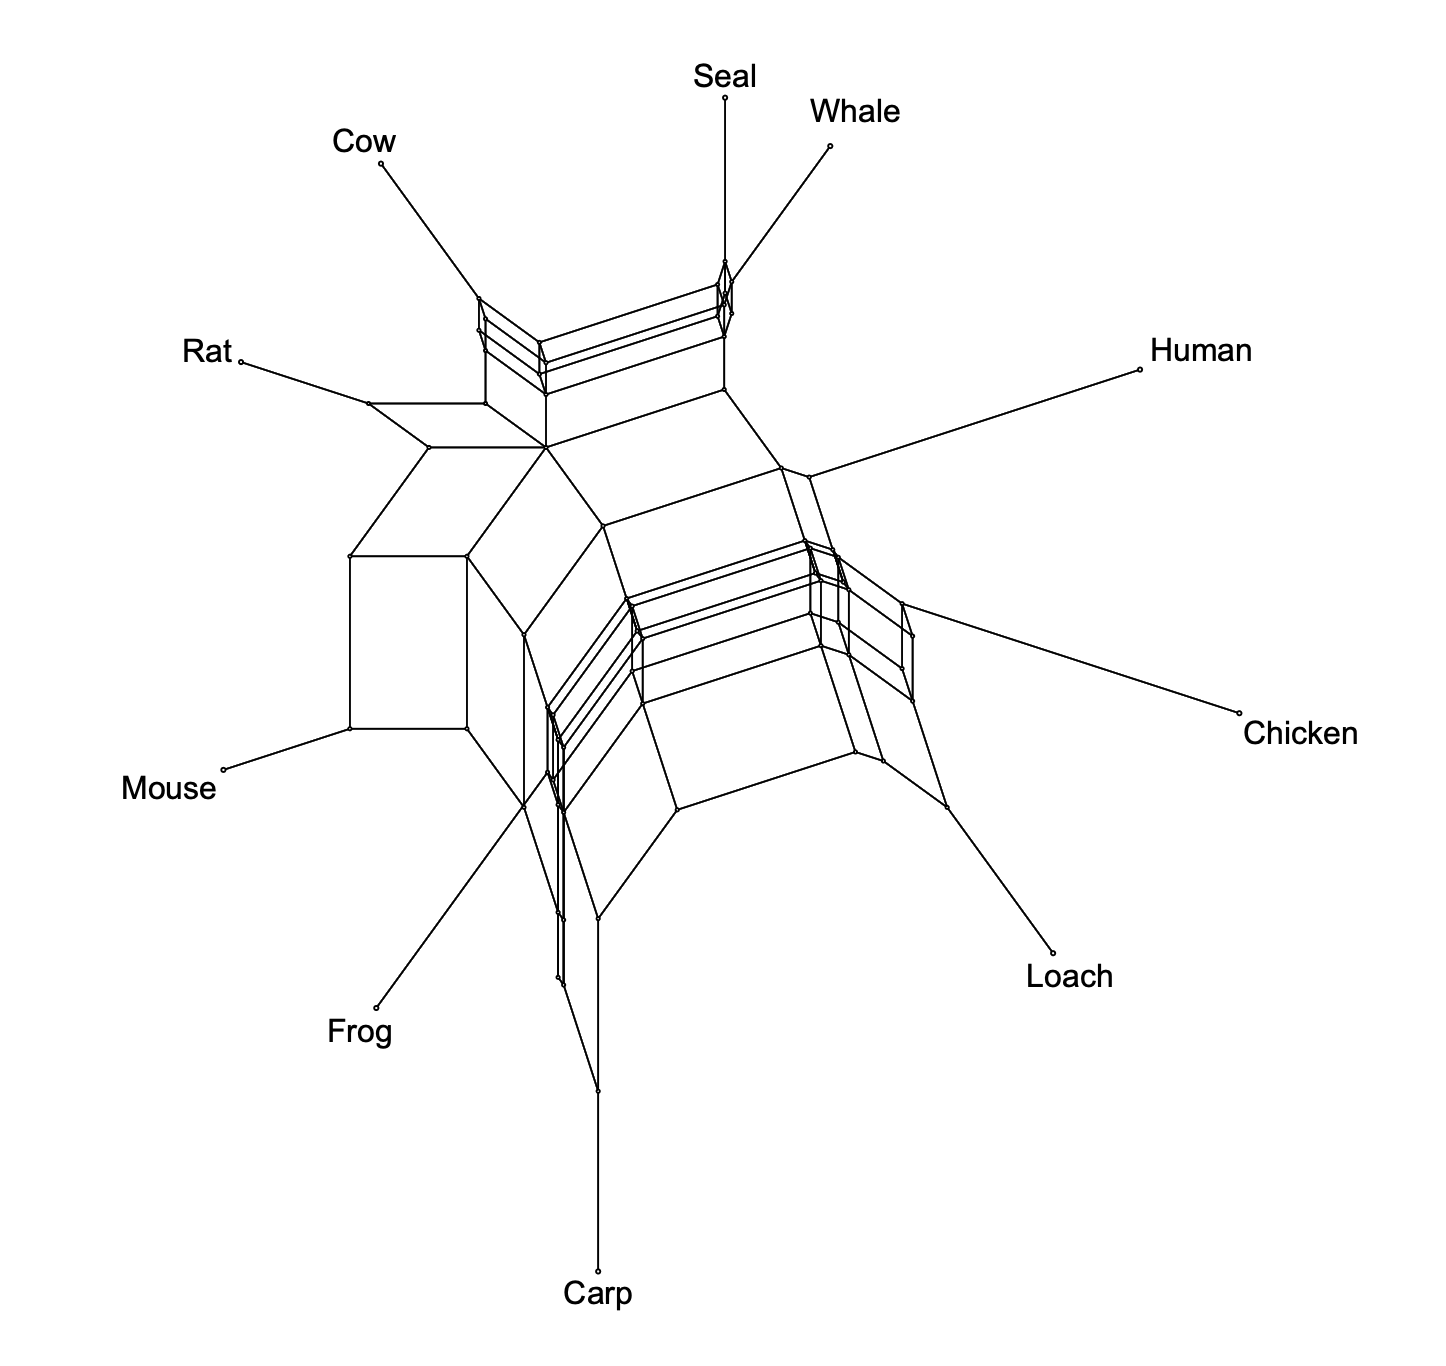
\includegraphics[width = 0.45\textwidth]{tree5.png}
		\end{figure}
		\noindent The strength of the splits network is the clear depiction of possible distances and features in which the calculation is highly confident. In the DensiTree Visualization however, one can see the confidence of different tree topologies by the number of lines forming this tree. This also holds for sub-trees or other features of the tree, and is missing in the splits network. However, the DensiTree visualization does not clearly show predicted edge lengths, because all predictions are superimposed. The probably most prominent difference is that one visualization is rooted, while the other is not. 				
\end{document}






